\setcounter{section}{18}
\section{Exam 2018/19}
{
\renewcommand{\thesubsubsection}{\thesubsection\alph{subsubsection}}
\subsection{Exercise 1}
\begin{center}    
    \begin{longtable}{c | c p{132mm}}
        \textbf{(a)} & True & \textbf{Circular wait} is one of the four conditions necessary for a deadlock, so removing circular waits is usually the best way to solve the deadlock, assuming all the other three conditions (mutual exclusion, hold and wait and no preemption) are unavoidable, which usually are in a scenario where sharing resources is absolutely necessary. \\
        \textbf{(b)} & True &
        \begin{minipage}{0.48\textwidth}
            Let $P_n$ be a process, where $n$ is the value of $i$ after incrementing and before evaluating the \textbf{for}-loop conditional. At each \texttt{fork}, \textbf{a new process is split into a parent and a child}. $P_4$ are the processes that will print \texttt{Hello}, since those will break the loop. Since there are eight $P_4$ processes, \texttt{Hello} will be printed eight times.
        \end{minipage}%
        \begin{minipage}{0.34\textwidth}
            \begin{tikzpicture}
                \Tree	[.$P_1$
                            [.$P_2$
                                [.$P_3$
                                    $P_4$
                                    $P_4$
                                ]
                                [.$P_3$
                                    $P_4$
                                    $P_4$
                                ]
                            ]
                            [.$P_2$
                                [.$P_3$
                                    $P_4$
                                    $P_4$
                                ]
                                [.$P_3$
                                    $P_4$
                                    $P_4$
                                ]
                            ]
                        ]
            \end{tikzpicture}
        \end{minipage} \\
        \textbf{(c)} & False & \textbf{\texttt{exec} calls do not create new processes}, they load another program's code into the current process and execute it, so the process code is only replaced. The calls corresponding to the problem statement are \texttt{popen} and \texttt{system}. \\
        \textbf{(d)} & True & It only makes sense to talk about \emph{quantum} when we are using round-robin (RR) scheduling, so we assume there are at least two \textbf{Multilevel Feedback Queue (MLQ)} queues which internally implement RR. Processes with higher priority are expected to finish execution faster, so they are assigned a smaller \emph{quantum}; if the assumption is not true then they have the wrong priority, and are moved to less-priority queues. \\
        \textbf{(e)} & \textcolor{red}{True} & \textbf{Preemption} usually uses a timer to keep track of time since it was last dispatched. Preemption usually also includes a system to interrupt a lower-priority process if a new process with higher priority arrives. \\
        \textbf{(f)} & False & A \textbf{\emph{race condition}} is a situation where two processes use the same data almost simultaneously, meaning the outcome may be highly unpredictable since it depends on the order of execution of each processes' instructions. It might lead to corrupted data if data is being simultaneously edited and read, or read by both processes. A \textbf{critical section} is a section of code that must be executed exclusively by one process at a time, so the fact two processes can't execute a critical section simultaneously is good, and usually achieved with a mutex. \\
        \textbf{(g)} & True & Two different processes can have the same \textbf{logical address} mapped to different \textbf{physical addresses}. Actually, it is also very likely that the virtual addresses of two processes sharing memory are different although they map to the same physical address. \\
        \textbf{(h)} & \textcolor{red}{False} & The \textbf{principle of locality of reference} states that there is a tendency that a program's instructions and data are repetitively accessed over a short period of time. This principle is not a base for virtual memory management, since its fundamental application would mean a process's code and data would be completely loaded into physical principal memory, and virtual memory is a way of seeming to have more virtual memory than physical memory, meaning instructions and data must be constantly swapped in and out of physical principal memory. \\
        \textbf{(i)} & False & \textbf{Multiprogramming} means there can be several processes loaded in principal memory simultaneously, while \textbf{multiprocessing} means several processes can run simultaneously. There can be multiprogramming without multiprocessing if it is possible to have multiple processes loaded in principal memory but only one process can be run at the same time (e.g., a virtual machine assigned with one running thread and 4GB of physical principal memory can have several loaded processes but only one can run at a time). \\
        \textbf{(j)} & False & After reading the last \textbf{directory entry}, \texttt{readdir} signals there are no more entries by returning \texttt{NULL}. \\
        \textbf{(k)} & False & \texttt{exec} calls do not create processes, they replace the current process running code. \\
        \textbf{(l)} & \textcolor{red}{False} & \texttt{ps} reports \textbf{current processes}, so it has nothing to do with signals. \\
        \textbf{(m)} & False & \textbf{i-nodes} do not contain file names, only directories contain (filename, inode) pairs. That is why several hard links to the same file can have different names. \\
        \textbf{(n)} & True & When a process is forked, all open file entries are duplicated automatically so the child process can use the same file without having to open it again (file pointers are also duplicated as a consequence, so file reads will not be synchronized between the parent and child processes). \\
        \textbf{(o)} & True & The \textbf{Process Control Block} holds essential information that must be available for retrieval by its parent, so the PCB may only be destroyed once that information has been retrieved by the parent. \\
        \textbf{(p)} & True & A system with 32-bit logical addresses can represent $2^{32}$ addresses; since each address maps to a byte, the total memory is $2^{32}\SI{}{\byte}=\SI{4}{\giga \byte}$. Pages have size $\SI{16}{\kilo \byte}=2^{14}\SI{}{\byte}$. This means \textbf{the page table has $2^{32}/2^{14}=2^{18}$ elements}. \\
        \textbf{(q)} & True & There are little guarantees to several similar signals being all received. In practice, we determined only two consecutive similar signals can be received, so the third signal sent while the first signal is being processed does not even arrive. \\
        \textbf{(r)} & True & In Linux, a thread function must have a prototype \texttt{void* f(void*)}. \\
        \textbf{(s)} & \textcolor{red}{False} & Using \texttt{sem\_open}, \texttt{sem\_close} and \texttt{sem\_unlink}, processes can create \textbf{named mutexes}, allowing two different processes to use the same, shared mutex. Besides, if an unnamed mutex is allocated in a memory region shared among several processes it might also be accessible. \\
        \textbf{(t)} & False & A piece of code that must be executed rapidly and without interruptions is an \emph{atomic} section. A critical section is one that must only be executed by one process/thread at a time, but there is no limitation as for interruptions, since the CPU may interrupt a process inside a critical section to run a completely unrelated process.
    \end{longtable}
\end{center}
\subsection{Exercise 2}

\subsubsection{Item a}
It makes no sense to initialize a semaphore with a negative value, since a semaphore aims at describing an amount of available resources that can be simultaneously consumed. If the initial semaphore value is negative, not only it breaks the logic by stating that initially there are already more resources being used than they should, but also by breaking the runtime logic that threads must \texttt{sem\_wait} to use a resource and \texttt{sem\_post} to unlock the resource; any thread aiming at using one of the resources controlled by that semaphore will be stuck in an eternal \texttt{sem\_wait} call, since no thread should call \texttt{sem\_post} to unlock a resource it does not own.

\subsubsection{Item b}
Semaphores \texttt{sem1} and \texttt{sem2} keep the number of times \texttt{doWork1} and \texttt{doWork2} may run. Only \texttt{doWork1} may run initially (\texttt{init(sem1, 1)}, \texttt{init(sem2, 0)}); each time a process is about to run its \texttt{doWork} function, it asks if it can still run by waiting for the respective semaphore; once it is done, it has exhausted its possibility to run but informs the other process that it has gained an opportunity to run (\texttt{P1} signals \texttt{sem2} and vice-versa).
\begin{lstlisting}[language=C]
/// P0
init(sem1, 1);
init(sem2, 0);
\end{lstlisting}
\begin{center}
\begin{minipage}{0.47\textwidth}\begin{lstlisting}[language=C]
/// P1
while(goOn){
    wait(sem1);
    doWork1();
    signal(sem2);
}
\end{lstlisting} \end{minipage} \hspace{2em}
\begin{minipage}{0.47\textwidth} \begin{lstlisting}[language=C]
/// P2
while(goOn){
    wait(sem2);
    doWork2();
    signal(sem1);
}
\end{lstlisting} \end{minipage}
\end{center}

\subsection{Exercise 3}

\subsubsection{Item a}
For simplicity and without loss of generality, let time be measured in integers, starting in $0$ and increasing by $1$ for each page being referred. In the second column, the contents of the frames are represented, where the first number is the page, and the second number is the last time it was referenced (so 1(4) means page 1 is in memory and was last referenced in time $t=4$).
\begin{center}
\begin{tabular}{l | c | l}
    \textbf{Processed} & \textbf{In memory} & \textbf{Comments} \\ \hline
    1 2 3 4            & 1(0) 2(1) 3(2) 4(3)     & No pages were loaded, pages 1, 2, 3, 4 swapped in \\
    1                  & 1(4) 2(1) 3(2) 4(3)     & No page faults \\
    5                  & 1(4) 5(5) 3(2) 4(3)     & Page fault, page 2 swapped out, page 5 swapped in \\
    4 3                & 1(4) 5(5) 3(7) 4(6)     & No page faults \\
    6                  & 6(8) 5(5) 3(7) 4(6)     & Page fault, page 1 swapped out, page 6 swapped in \\
    5                  & 6(8) 5(9) 3(7) 4(6)     & No page faults \\
    1                  & 6(8) 5(9) 3(7) 1(10)    & Page fault, page 4 swapped out, page 1 swapped in \\
    3                  & 6(8) 5(9) 3(11) 1(10)   & No page faults \\
    2                  & 2(12) 5(9) 3(11) 1(10)  & Page fault, page 6 swapped out, page 2 swapped in \\
    4                  & 2(12) 4(13) 3(11) 1(10) & Page fault, page 5 swapped out, page 4 swapped in \\
    6                  & 2(12) 4(13) 3(11) 6(14) & Page fault, page 1 swapped out, page 6 swapped in \\
    1                  & 2(12) 4(13) 1(15) 6(14) & Page fault, page 3 swapped out, page 1 swapped in \\
    5                  & 5(16) 4(13) 1(15) 6(14) & Page fault, page 2 swapped out, page 5 swapped in \\
    2                  & 5(16) 2(17) 1(15) 6(14) & Page fault, page 4 swapped out, page 2 swapped in \\
    4                  & 5(16) 2(17) 1(15) 4(18) & Page fault, page 6 swapped out, page 4 swapped in
\end{tabular}
\end{center}
There were 14 page faults.

\subsubsection{Item b}
\textbf{(1)} One can find a process started thrashing when it finds almost as many page faults as references.\\
\textbf{(2)} Thrashing happened in the sequence 2 4 6 1 5 2 4.

\subsubsection{Item c}
\textbf{(1)} The process started thrashing because the number of actively used pages (5 pages: 1, 2, 4, 5, 6) is larger than the number of allocated frames (4), and because the LRU strategy is not optimal.\\
\textbf{(2)} One could use the page fault rate strategy, which starts by making an assumption as to what is an acceptable range of page fault rates, and after monitoring the page fault rate of each process during a certain time interval it performs frame allocations/deallocations to processes:
\begin{itemize}
    \item Allocates an additional frame if the process has more page faults than acceptable.
    \item Deallocates one of its frames if the process has less page faults than acceptable (these frames can then serve other processes).
\end{itemize}

\subsection{Exercise 4}

\textbf{(1)} Unix supports files of various sizes. This is achieved using indexed file allocation, which consists of keeping, for each file, a special block containing its metadata and a table of all blocks allocated to that file. This strategy has many advantages, namely allowing fast modification and reduced external fragmentation (compared to contiguous allocation), as well as relatively fast direct access and added reliability (compared to linked allocation). To allow fast file expansion, Linux file systems uses direct indexes combined with multilevel indexes, where smaller indexes point directly to file blocks, and higher indexes point to other index blocks of growing depth. This allows fast access to small files (since their blocks are directly indexed), while also allowing decent performance when using large files (since they are indexed in a sort of logarithmic way).\\
\textbf{(2)} Say an index can be interpreted as a reference. On accessing very large files, even on accessing small portions of the end of a large file, there is a need to dereference all the numerous indexes from index block to index block before finding the block we are looking for, since the lowest indexes require less dereferencing (memory blocks are more directly indexed) than higher indexes.

\subsection{Exercise 5}
\lstinputlisting[language=C,basicstyle=\footnotesize]{2019N_05.c}

\subsection{Exercise 6}
\subsubsection{Item a}
The FIFO must be created by the reader process, since it acts as the server and provides services to other processes that might know how to communicate with it. Since the FIFO serves the purpose of receiving messages for the reader to process, it only makes sense for the FIFO to exist as long as the reader is running.

\subsubsection{Item b}
\begin{lstlisting}[language=C]
mkfifo("/users/tmp/srvfifo", 0000);
\end{lstlisting}

\subsubsection{Item c}
Writes of up to \texttt{PIPE\_BUF} bytes are guaranteed to be atomic, so it is impossible for two messages to overlap on writting.\par
As for reads, there is no atomicity guarantee, so there is a chance reads are interleaved. However, common sense tells there is no chance to read the same message twice, since once a character is read once it is removed from the FIFO and cannot be read again by another process. So in the terms of the problem statement it is impossible to read the same message twice.\par
If interleaved reading is considered a problem, it can be solved using a named mutex to enforce mutually exclusive reads.\par
As an alternative, a message queue could be used.

\subsubsection{Item d}
\textbf{(1)}
\begin{lstlisting}[language=C]
/// Reader
int main(){
    int mem = shm_open("/tmp/is_fifo_open", O_CREAT|O_RDWR, 0600);
    ftruncate(mem, sizeof(int));
    int *is_fifo_open = mmap(NULL, sizeof(int), PROT_READ|PROT_WRITE,
                             MAP_SHARED, mem, 0);
    *is_fifo_open = 1;
    char message[8192];
    while(readfifo_nonblock(message) == 0){
        process(message);
        if(should_close_fifo()){ *is_fifo_open = 0; break; }
    }
    while(readfifo_nonblock(message) == 0) process(message);
    munmap(mem, sizeof(int)); shm_unlink("/tmp/is_fifo_open");
    return 0;
}
\end{lstlisting}
\begin{lstlisting}[language=C]
/// Writter
int main(){
    int mem = shm_open("/tmp/is_fifo_open", O_RDONLY, 0600);
    int *is_fifo_open = mmap(NULL, sizeof(int) ,PROT_READ,
                             MAP_SHARED, mem, 0);
    char message[8192];
    while(has_messages_to_write()){
        create_message(message);
        if(*is_fifo_open) writefifo(message);
        else break;
    }
    munmap(mem, sizeof(int));
    return 0;
}
\end{lstlisting}

\textbf{(2)}
\begin{lstlisting}[language=C]
/// Reader
int fifo_filedes;
int openfifo_nonblock(){
    mkfifo("/tmp/fifo", 0600);
    fifo_filedes = open("/tmp/fifo", O_RDONLY|O_NONBLOCK, 0600);
}
int readfifo_nonblock(char *message){
    int r = read(fifo_filedes, message, 8192);
    if(r != 8192) return 1;
    return 0;
}
\end{lstlisting}
\textbf{(3)}
A writter could know it cannot write to the FIFO any longer by checking the value of the integer in shared memory \texttt{/tmp/is\_fifo\_open}.

\subsection{Exercise 7}
\subsubsection{Item a}
The usage of \texttt{arg[]} is justified because each thread must receive its own individual index, where each index is in a different memory address, to make it persistent and allow different indexes for different threads. Otherwise, if we used the cycle variable, not only would it sooner or latter become out-of-scope (after the cycle ends) and cause undefined behaviour in the threads, but even if it was defined in the heap we would be providing all threads the same pointer, meaning all threads would think they had the same \texttt{thrIndex}.

\subsubsection{Item b}
If \texttt{main()} ended with \texttt{exit(0)}, the whole process would be terminated, including all threads. With \texttt{pthread\_exit(NULL)}, only the main thread is terminated, and the threads that were just launched continue running inside the original process.

\subsubsection{Item c}
It is made with blocking, since a thread waits by locking \texttt{mutex}, which is a blocking call. However, for each \texttt{numThreads} times a thread acquires the lock, it only performs useful work once. This can in some cases be considered busy-wait, particularly if the number of threads is large.

\subsubsection{Item d}
\begin{lstlisting}[language=C]
#include <stdio.h>
#include <unistd.h>
#include <stdlib.h>
#include <pthread.h>

pthread_mutex_t mutex = PTHREAD_MUTEX_INITIALIZER;
int numThreads;
int turn = 0; // The first thread to run must have thrIndex=turn=0
pthread_cond_t *conds = NULL;                               // <========

void * thr(void *arg){
    int thrIndex = *(int*)arg; // The effective indexes are 0,1,2,...
    while (1){
        pthread_mutex_lock(&mutex);
        while(thrIndex != turn)                             // <========
            pthread_cond_wait(conds[i], &mutex);            // <========
        printf("%d ", thrIndex + 1);                        // <========
        turn = (turn + 1) % numThreads;                     // <========
        pthread_mutex_unlock(&mutex);
    }
    return NULL;
}
int main(){
    printf("Number of threads ? "); scanf("%d", &numThreads);
    int *arg = (int *) malloc(sizeof(int)*numThreads);
    conds = calloc(numThreads, sizeof(pthread_cond_t));     // <========
    pthread_cond_signal(conds[turn]);                       // <========
    pthread_t *tid = (pthread_t *) malloc(sizeof(pthread_t)*numThreads);
    for (int i = 0; i < numThreads; i++){
        arg[i] = i;
        pthread_create(&tid[i], NULL, thr, (void*)&arg[i]);
    }
    pthread_exit(NULL);
}
\end{lstlisting}

}
